\documentclass[12pt,oneside,openany,letterpaper]{article}


\usepackage{fancyhdr}
\usepackage{helvet}
\usepackage{amsmath}
%\usepackage{graphicx}
\usepackage[pdftex]{graphicx}
\usepackage{psfrag}
\usepackage{setspace}
%\usepackage[hypertex, linktocpage]{hyperref}[2003/11/30]
\usepackage[linktocpage]{hyperref}[2003/11/30]
\usepackage{lscape}
\usepackage{nicefrac}
\usepackage{mathrsfs}
\usepackage{units}
\usepackage{upgreek}
\usepackage{amssymb}
\usepackage{color}
\usepackage{wrapfig}
\usepackage{multirow}
\usepackage{url}
\usepackage{verbatim}
\usepackage{textcomp}
\usepackage{epstopdf}

\onehalfspacing \setlength\textheight{667pt}
\setlength\textwidth{506pt} \setlength\oddsidemargin{-18pt}
\setlength\topmargin{-20pt}
%\setlength\footskip{24pt}
\addtolength\headheight{2.5pt} \addtolength\headsep{-14pt}
%\fancyhead[R]{\includegraphics[height=10.5pt]{ubclogo_bw.eps}\#:  55907968}
%\renewcommand\familydefault{\sfdefault}
\pagestyle{empty}

\newenvironment{packed_enum}{
\begin{enumerate}
  \setlength{\itemsep}{0pt}
  \setlength{\parskip}{0pt}
  \setlength{\parsep}{0pt}
}{\end{enumerate}}



\fancyhead[L]{\emph{Introduction to Electronics}}\fancyhead[R]{$LRC$ Transients and Resonance}
\fancyfoot[L]{PHYS 231}\fancyfoot[R]{Experiment 4}
\pagestyle{fancy} \pagenumbering{arabic}

\begin{document}
\thispagestyle{plain}
\begin{center}
{\large{\bf{\fontfamily{phv}\selectfont Physics 231 - AC \& Transient Response of an $LRC$ Circuit (Exp.~4)}}}
\end{center}

\noindent This experiment is intended to provide you with a working knowledge of some of the basic properties of a resonant $LRC$ circuit, both its transient response and its frequency response. It also provides you with an introduction to nonlinear least-squares fitting.

~


{\bf INTRODUCTION}

~

\noindent The series $LRC$ circuit shown in Fig.~\ref{fig:fig1} is an example of the simplest damped resonant system, known as the damped harmonic oscillator. If the ac source produces a sinusoidal signal with amplitude $V_0$ and angular frequency $\omega$, then the ratio of the voltage amplitude across the resistor to the voltage amplitude across the ac source is:
\begin{equation}
\frac{V_R}{V_0}=\frac{1}{\sqrt{1+\left(\omega\dfrac{L}{R}-\dfrac{1}{\omega RC}\right)^2}}\label{eq:peak}
\end{equation}
The resonant frequency and bandwidth of this harmonic oscillator are:
\begin{align}
\omega_0&=\frac{1}{\sqrt{LC}}\\
\gamma&=R/L
\end{align}
You will find it convenient to rewrite the voltage ratio in terms of these two quantities, which will give you an important expression for the frequency response of a resonant system (also known as a Lorentzian lineshape).  Further details on the $LRC$ circuit can be found in almost any basic text on ac circuits.
\begin{figure}[b!]
\begin{center}
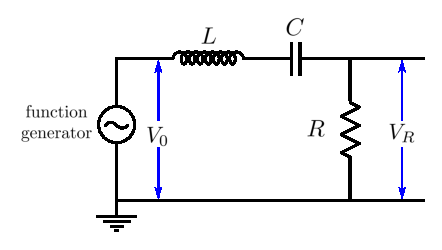
\includegraphics[width=.58\textwidth]{LRC.eps}\caption{\label{fig:fig1}The series $LRC$ circuit.}
\end{center}
\end{figure}
\clearpage


{\bf 1. TRANSIENT RESPONSE}

~

\noindent Assemble the series $LRC$ circuit shown in Fig.~\ref{fig:fig1} using the component values \mbox{$L=20$~mH}, \mbox{$C=0.001~\upmu$F}, and \mbox{$R=1000~\Omega$}.

~

\noindent Investigate the transient response by applying low frequency \emph{square waves} from the function generator and using the oscilloscope to observe the voltage across the resistor $V_R$. You should observe damped harmonic oscillations in $V_R(t)$. Measure both the frequency of the oscillations $\omega_1$ and the time constant $\tau$ that governs the exponential damping of the amplitude of the oscillations. You should collect enough points in the exponential decay to perform a linear least-squares fit to determine $\tau$.

~

{\bf 2. FREQUENCY RESPONSE}

~

\noindent To investigate the ac frequency response of the resonant circuit, you should switch the generator to \emph{sinusoidal output} and observe both $V_0$ and $V_R$ on the two channels of the oscilloscope. Measure both the phase and amplitude of $V_R$ relative to $V_0$ over a frequency range wide enough to clearly show the resonant behaviour (1~kHz -- 70~KHz). Pay particular attention to the frequencies in the vicinity of the resonance peak. There are three points of great importance: the resonant frequency where $V_R$ reaches its maximum value, and the two points on either side of the resonance where $V_R/V_0 = 1/\sqrt{2}$ and the phase shift is $\pm 45^\circ$.

~

\noindent Use your measurements to plot $V_R /V_0$ versus $\omega$ and then determine, by fitting a Lorentzian curve to the data, the resonant frequency, $f_0$, of this circuit (where $\omega_0=2\pi f_0$) and the bandwidth $\gamma$. The dependence of $V_R /V_0$ on $\omega$ is clearly nonlinear.  For this curve-fitting task (again weighted by the errors in the measured data), you will be using the nonlinear least squares fitting function of Maple (or any suitable data analysis software of your choice).  After re-expressing Eq.~\ref{eq:peak} in terms of $\omega_0$ and $\gamma$, try fitting your data to the resulting expression.  Leave $\omega_0$ and $\gamma$ as unknown parameters to be determined by the fitting routine. If the fit is unsatisfactory, you may need to include a third fitting parameter to adjust the height of the peak. Try to explain why this third parameter is needed. Compare the resonant frequency and damping to the results obtained in part 1 in order to determine the relationship between the transient response and the ac response.

~

\noindent {\bf You have two 3-hour periods to complete this lab.  Therefore, you are expected to collect lots of high-quality data and complete a thorough analysis.}  You should collect the data \emph{and} complete as much of the analysis as possible during lab time.  


\end{document}
